\documentclass[letterpaper,10pt]{article}

%\setlength{\parindent}{0in}
%\usepackage{fullpage} 
\usepackage{amsmath}
\usepackage{amssymb}
\usepackage{enumerate}
\usepackage{graphicx}
\usepackage[table]{xcolor}
\usepackage{dcolumn}
\usepackage[english]{babel}
\oddsidemargin 0.0in
\textwidth 6.5in
\newcolumntype{.}{D{.}{.}{-1}}
\newcommand*{\myalign}[2]{\multicolumn{1}{#1}{#2}}
% Alter some LaTeX defaults for better treatment of figures:
    % See p.105 of "TeX Unbound" for suggested values.
    % See pp. 199-200 of Lamport's "LaTeX" book for details.
    %   General parameters, for ALL pages:
    \renewcommand{\topfraction}{0.9}	% max fraction of floats at top
    \renewcommand{\bottomfraction}{0.8}	% max fraction of floats at bottom
    %   Parameters for TEXT pages (not float pages):
    \setcounter{topnumber}{2}
    \setcounter{bottomnumber}{2}
    \setcounter{totalnumber}{4}     % 2 may work better
    \setcounter{dbltopnumber}{2}    % for 2-column pages
    \renewcommand{\dbltopfraction}{0.9}	% fit big float above 2-col. text
    \renewcommand{\textfraction}{0.07}	% allow minimal text w. figs
    %   Parameters for FLOAT pages (not text pages):
    \renewcommand{\floatpagefraction}{0.7}	% require fuller float pages
	% N.B.: floatpagefraction MUST be less than topfraction !!
    \renewcommand{\dblfloatpagefraction}{0.7}	% require fuller float pages


\title{Project 1}
\author{Douglas Brown \\ Jessica Hale \\ Steve Mazza \\ Daniel Torres}
\date{February 1, 2012}

\begin{document}
\maketitle
\tableofcontents
\listoffigures
\listoftables
\pagebreak

\begin{abstract}
We consider two historical battles, the first of which is the Battle of Cajamarica which pits Spanish forces led by Francisco Pizarro against a much larger Inca army directed by the Emperor Atahuallpa.  We know from history that the much larger Inca army did not fare well against the technologically superior albeit much smaller Spanish forces.

The second conflict that we consider is the Battle at Little Bighorn.  This sees COL Custer's defeat against an overwhelming Sioux presence.  The stark contrast of the outcome of these two conflicts helps us to understand the respective roles and gravity of technological superiority and sheer force strength in shaping the outcome of battle.

Using the modeling and simulation environment, ExtendSim, we investigate the effects of tactics and technology on these historical battles, focusing closely on surprise tactics and the use of modern weaponry, armor, and mobility to defeat larger forces.

We determine that technological superiority is necessary to overcome a deficit in number but that it must be both sufficiently great and maintained throughout the engagement.
\end{abstract}

\section{Ancient Warfare: Battle of Cajamarca}
%TODO: Write brief introduction.

\subsection{Requirement 1}
Lanchester's Linear Law as applied to the battle of Cajamarca is described by two differential equations (with the variable $S$ denoting the Spanish forces and the variable $I$ denoting the Incan forces).

Note that since the Incas were not successful in killing even a single Spaniard -- the $a$-coefficient (Incan attrition rate) is zero for the model that replicates the historical battle.  The linear law is applied here due to the weapons in use at the time; the largest individual combatant battle spaces at the scene would have been limited to a relatively small circular area around the Spanish mounted cavalry

Given:
\begin{align*}
\frac{dS}{dt} &= -a\times S(t)\times I(t) \\
\frac{dI}{dt} &= -b\times S(t)\times I(t)
\end{align*}
With initial conditions $S(0) = S_{0}$ and $I(0) = I_{0}$, the formula for the $S$-force is:
\begin{equation}\label{eq1}
S(t) = S_{0}\left(\frac{bS_{0}-aI_{0}}{bS_{0}-aI_{0}e^{aI_{0}-bS_{0}t}} \right)
\end{equation}
for $bS_{0}\neq aS_{0}$ or,
\begin{equation}\label{eq2}
S(t) = \frac{S_{0}}{1+bS_{0}t}
\end{equation}
for $bS_{0}=aS_{0}$.  The formula for the $I$-force is:
\begin{equation}\label{eq3}
I(t) = I_{0}\left(\frac{aI_{0}-bS_{0}}{aI_{0}-bS_{0}e^{-(aI_{0}-bS_{0})t}} \right)
\end{equation}
for $bI_{0}\neq aI_{0}$ and
\begin{equation}\label{eq4}
I(t) = \frac{I_{0}}{1+aI_{0}t}
\end{equation}
for $aI_{0} = bI_{0}$.  Since $a=0$ and 7000 Incas were killed we will use equations \eqref{eq1} and \eqref{eq3}.  It follows that
\begin{align*}
S(t) &= S_{0}\left(\frac{bS_{0}}{bS_{0}} \right) \\
&= S_{0} \\
&= 168
\end{align*}
\begin{align*}
I(t) &= I_{0}\left(\frac{-bS_{0}}{-bS_{0}e^{-(-bS_{0})t}} \right) \\
&= I_{0}\left(\frac{1}{e^{bS_{0}t}} \right) \\
e^{bS_{0}t} &= \frac{I_{0}}{I(t)} \\
bS_{0}t &= \ln\left(\frac{I_{0}}{I(t)} \right) \\
b &= \frac{\left(\ln\left(\frac{I_{0}}{I(t)}\right) \right)}{S_{0}t}
\end{align*}
Given $I(480) = 73000$ and $S_{0} = 168$,
\begin{align*}
b &= \frac{\ln\left(\frac{80000}{73000} \right)}{168\times 480} \\
&= 1.136\times 10^{-6} \\
&\approx 0.000001135
\end{align*}
This can be interpreted as an average number of Incas killed per minute per (number of Incas multiplied by number of Spaniards).

\subsection{Requirement 2}
The battle of Cajamarca , fought 16 November 1532 in present-day Peru between the Inca Emperor Atahuallpa (with 80,000 Indian infantry) against Francisco Pizarro (with 168 Spaniards:  62 cavalry and 106 infantry).  In eight hours, it is estimated that the Spanish killed 7000 Inca and captured the Emperor, without losing a single man.

Armaments for the forces were quite different.  The Incas were armed with clubs and stone hatchets.  They wore quilted \emph{armor}.  The Spaniards had steel helmets and body armor, and steel swords and lances.  The Indian quilted armor was effective against blunt instruments such as clubs, but offered little protection against piercing by steel swords and lances.  The Spaniard armor was quite effective against the Indians' primitive weapons.

Though the Spanish forces were greatly outnumbered, many Inca warriors had never encountered horses before; they were described as having a mythical beast kind of reputation.  The decision by Atahuallpa to leave most of the 80,000 warriors outside the city walls was one that worked decidedly in favor of the Spanish.  Though Atahuallpa understood he was hosting other men, unlike his Aztec counterpart Montezuma who considered the Spaniards to be deities, he appeared to have misunderstood the risk and threat that he and his warriors and security attachment faced in the meeting with Pizarro and deSoto that day.  Pizarro apparently recalled and recounted the successful tactic of capturing the emperor employed by his counterpart Cortez against the Aztecs when laying out the surprise battle plan for the following day.

\begin{figure}[h!tp]
\begin{center}
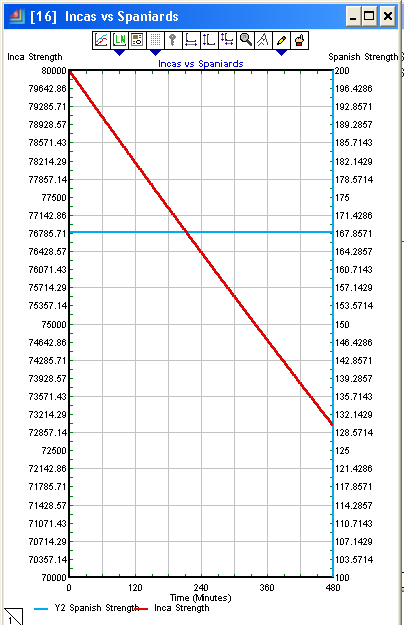
\includegraphics[scale=0.4]{fig2a.png}
\caption{Spanish vs. Inca forces}
\label{fig2a}
\end{center}
\end{figure}

The ExtendSim model that replicates the battle shows a quick attrition of the Incas by the Spaniards that was better described as a massacre due to the very light armor and lack of weapons the Incas present inside the city walls at Cajamarca possessed that day.  See Figure \ref{fig2a}.  The model shows the somewhat linear decay of the attrition rate, starting at slightly more than 1,000 per hour at the commencement of the attack and falling off to less than 1,000 per hour at the end of the fighting (due to the decreasing number of Inca warriors).  Descriptions of the account point to a possibly higher initial attrition rate since the surprise attack began with a cavalry charge and gunfire by hidden Spanish troops.  A small battery of cannon also contributed to the high attrition rate achieved by the Spanish as well as accounts of Incas sacrificing their lives in hopes of saving their emperor.

\subsection{Requirement 3}
\subsubsection{Development}
The ExtendSim fixed step model created uses kill efficiency constant blocks that are inputs to a multiplication math block that applies the other two inputs of the Spanish force strength and Inca force strength in one minute time steps to permit subtraction of forces from each of the holding tank reservoir blocks that model the Spanish and Inca forces.  Those force strengths are output to a Plotter I/O to permit creation of a table and a graph depicting the decrease in force strengths as the battle progresses.  The actual battle conditions left the Spanish force strength constant at the initial strength of 168.  Altering the model account for an Inca attrition rate and variable Spanish force strength permitted excursions to analyze the possible effects of alternative Inca tactics.

\subsubsection{Results}
The simulation results from the model depict the fast attrition rate of the relatively defenseless Inca warriors who were unaccustomed to battle of this intensity with firearms, cannon, and armored mounted cavalry, the ground combat vehicles of the times.  7,000 Incas had been killed when the emperor was captured after eight hours, and accounts indicate that his life was saved from an attacking Spaniard by Pizarro.  Three excursions were studied in the simulation model – one with an Inca attrition coefficient of $\frac{1}{1000}$ the rate of the Spanish (see Figure \ref{fig3b}), one with an Inca attrition coefficient of $\frac{1}{100}$ the rate of the Spanish (see Figure \ref{fig3a}), and one with an Inca attrition coefficient of $\frac{1}{10}$ the rate of the Spanish (see Figure \ref{fig3c}).  The small improvement creates the unlikely result of the force strengths drawing even to just fewer than 90 after over a month of around the clock battle.  The larger theoretical Inca attrition rate actually creates a war of attrition potential success scenario for the Incas after less than five days of continuous around the clock battle, though at a heavy loss of almost 17,000 warriors.  Closer examination of the history and setting indicates that these are very unlikely results.

\begin{figure}[h!tp]
\begin{center}
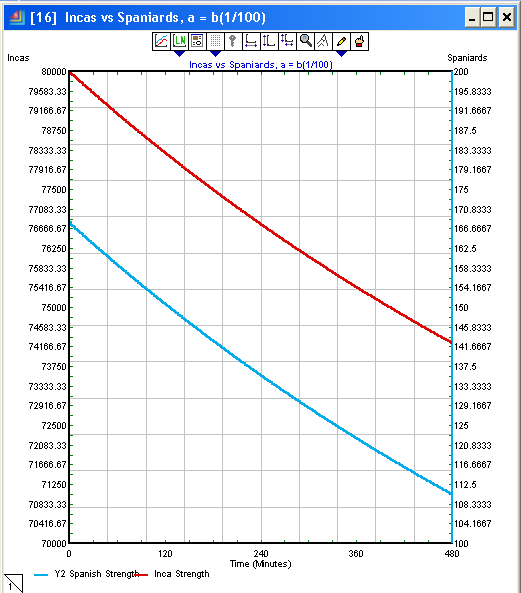
\includegraphics[scale=0.4]{fig3a.png}
\caption{Spanish vs. Inca forces, $b=\frac{1}{100}$}
\label{fig3a}
\end{center}
\end{figure}

\begin{figure}[h!tp]
\begin{center}
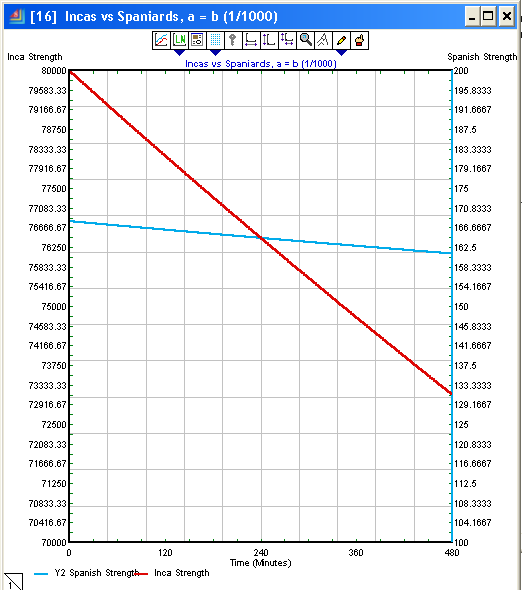
\includegraphics[scale=0.4]{fig3b.png}
\caption{Spanish vs. Inca forces, $b=\frac{1}{1000}$}
\label{fig3b}
\end{center}
\end{figure}

\begin{figure}[h!tp]
\begin{center}
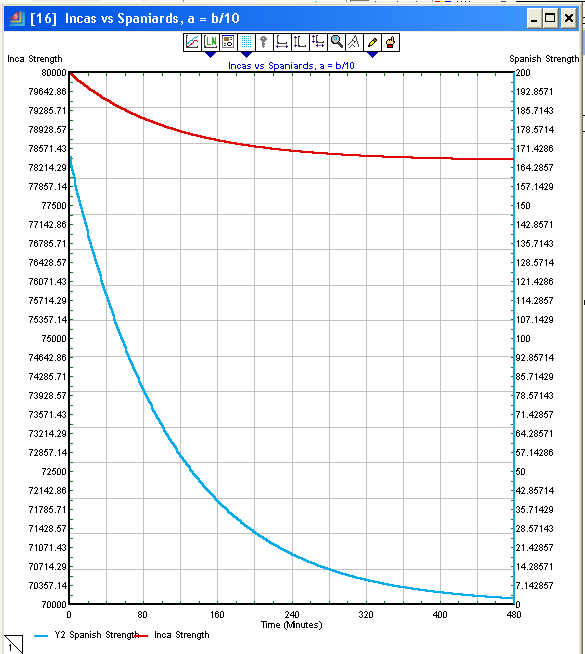
\includegraphics[scale=0.4]{fig3c.png}
\caption{Spanish vs. Inca forces, $b=\frac{1}{10}$}
\label{fig3c}
\end{center}
\end{figure}

Tactics always matter in a battle. The Spaniards utilized a form of warfare with which the Incas had no prior knowledge.  The weapons and armor the Spanish employed along with the use of cavalry left the Incas at a great disadvantage in the battle.  The Incas would have had to recognize they were over-matched and revolutionize their tactics on the initial day of fighting.  It is unreasonable to expect that they should have done this, so their loss was inevitable.

The Incas normally displayed their large and well trained army to an enemy and the enemy would surrender without a fight.  If fighting was required, it was done as hand to hand combat on open terrain with much of the Inca manpower used to flank. The mobility of the Spanish cavalry was critical in the battle.  Spanish cavalry mobility severely inhibited the Incas ability to flank, allowed the Spanish to break up Inca head-on attacks, and allowed the Spanish to quickly initiate successful attacks against the Incas.

It is critical that the Spanish did not demonstrate battle superiority and wait for the Incas to surrender.  They continued fighting until victory was achieved.  This left the Incas without the time required to develop completely new tactics.

To be more effective, the Inca tactics would have had to change significantly. The Incas should have brought the battle to more difficult terrain where the Spanish cavalry would be ineffective.  Eliminating the cavalry effectiveness by fighting in mountains or jungles may have allowed the Incas to surprise the Spanish and achieve some success.  In more rugged terrain, the Incas could have tried to attack the Spanish from above with rocks, spears, or arrows.  Difficult terrain may have made it possible for the Incas to break the Spaniards into smaller numbers where traditional attacks may have worked better.  Even with altered tactics, the Incas would have likely suffered huge casualties in the battles.

The Incas needed a more effective defense to protect troops and encampments from Spanish cavalry attacks.  They could have constructed trenches, walls, or barriers to prevent Spanish access.  This would have taken time that they did not have at the battle of Cajamarca.

In hindsight it appears that only one army planned for battle that day (or was familiar with battle planning as a concept).  Strategic and cultural changes would have been required for the Incas to somehow prevail during the battle.  Pizarro directed that the meeting would be held in the town square at Cajamarca, which effectively cutoff most of the Inca reinforcement warriors outside the city walls.  Pizarro's plan needed to work very effectively and with little tactical adjustment required on their part during the battle, as the nearest Spanish reinforcement units were 1,000 miles away.  Even if more warriors had been brought into the city square, one impact of this would have been an even higher Spanish attrition rate owing to the even higher density of Inca warriors, multiplying the effectiveness of their guns, cannon, and cavalry charges.  The Inca force impetus to protect the emperor (a living deity) at all costs, including self-sacrifice, also rendered many of the warriors ineffective that day.

\section{Modern Warfare: Battle at Little Bighorn}
\subsection{Requirement 4}
Both $a$ and $b$ are unit-less constants with values 0.01 and 0.03 respectively.  They are an aggregate measure of force strength for each side.  Modeling the battle in Extend for the scenario where all of the $7^{th}$ Cavalry attacks all of the Sioux at once produces the results shown in Figure \ref{fig4a}.

\begin{figure}[h!tp]
\begin{center}
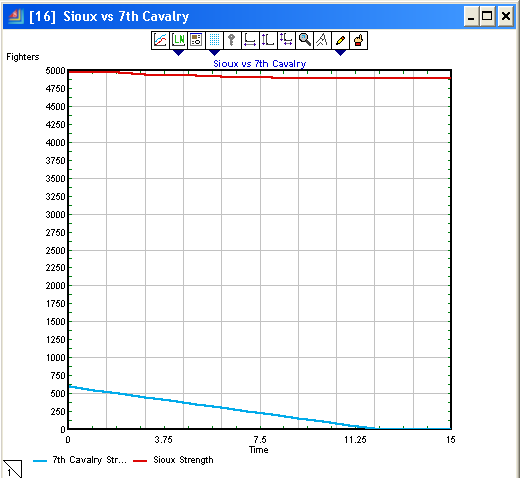
\includegraphics[scale=0.4]{fig4a.png}
\caption{$7^{th}$ Cavalry attacks Sioux \emph{en masse}}
\label{fig4a}
\end{center}
\end{figure}

As you can see from the results, the entire $7^{th}$ Cavalry is annihilated after twelve minutes and the resultant Sioux strength is 4,882.

\subsection{Requirement 5}
This model considers the case where General Custer divides his forces, placing 115 men under Major Reno.  The outcome shown in Figure \ref{fig5a} is somewhat different and more closely matches the historical data.
\begin{figure}[h!tp]
\begin{center}
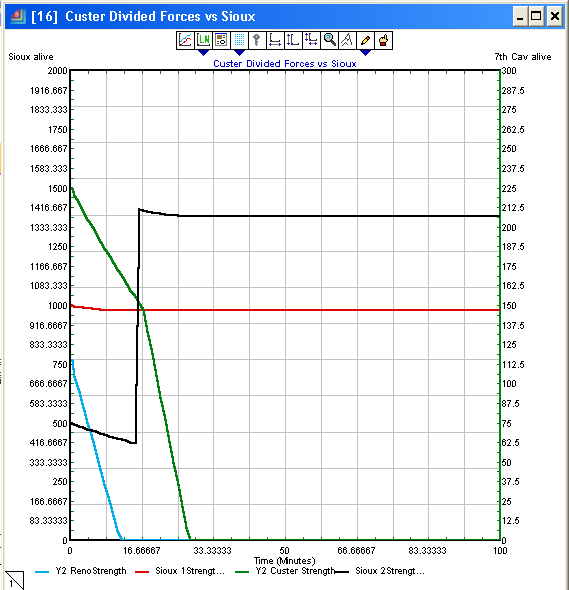
\includegraphics[scale=0.4]{fig5a.png}
\caption{$7^{th}$ Cavalry attacks Sioux divided}
\label{fig5a}
\end{center}
\end{figure}

Major Reno's forces survive for eleven minutes leaving 978 Sioux and General Custer's men survive for twenty-seven minutes leaving 1,379 for a combined Sioux strength of 2,357.

\subsection{Requirement 6}
Assume that a surprise attack by the $7^{th}$ Cavalry leads to an attrition coefficient that is no longer constant.   The element of surprise is considered to equate to a surprise coefficient of 20, which lasts for the initial 10 minutes of battle.  After the first 10 minutes of fighting, the element of surprise has lost impact and the coefficient returns to the original value.  This scenario assumes the battle follows the Lanchester Square Law without reinforcement with equations given by:

\begin{align*}
\frac{dB}{dt} &= -aR(t) \\
\frac{dR}{dt} &= -20bB(t) \mbox{\ for\ } t < 10 \\
\frac{dR}{dt} &= -bB(t) \mbox{\ for\ } t \geq 10
\end{align*}

Using the surprise coefficient, the results for the battle described in Requirement 4 can be recalculated.  In this scenario, the entire $7^{th}$ Cavalry surprises the Sioux with an en masse attack.  The results are shown in Figure \ref{fig6a} and Table \ref{tab6a}.
\begin{figure}[h!tp]
\begin{center}
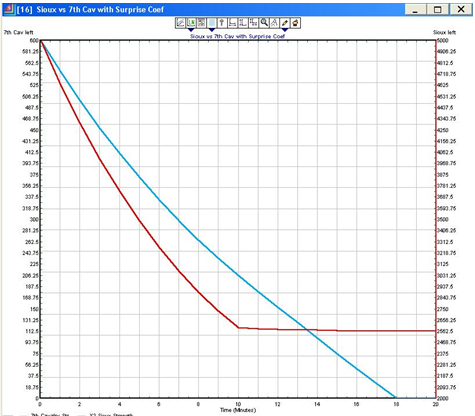
\includegraphics[scale=0.4]{fig6a.png}
\caption{$7^{th}$ Cavalry attacks Sioux \emph{en masse} with Surprise Coefficient}
\label{fig6a}
\end{center}
\end{figure}

\begin{table}
\begin{center}
\begin{tabular}[h!tp]{ccc}
\hline
\textbf{Time (minutes)} & \textbf{$7^{th}$ Cavalry Strength} & \textbf{Sioux Strength} \\
\hline\hline
0 &	600 &	5000 \\
1 &	550 &	4640 \\
2 &	500 &	4310 \\
3 &	453 &	4010 \\
4 &	410 &	3737 \\
5 &	370 &	3491 \\
6 &	333 &	3269 \\
7 &	298 &	3069 \\
8 &	265 &	2890 \\
9 &	234 &	2731 \\
10 &	205 &	2590 \\
11 &	178 &	2584 \\
12 &	152 &	2579 \\
13 &	126 &	2574 \\
14 &	100 &	2570 \\
15 &	75 &	2567 \\
16 &	49 &	2565 \\
17 &	23 &	2563 \\
18 &	0 &	2563 \\
\hline
\end{tabular}
\end{center}
\caption{$7^{th}$ Cavalry Attacks Sioux \emph{en masse} with Surprise Coefficient (data)}
\label{tab6a}
\end{table}

The battle lasts approximately 18 minutes before the $7^{th}$ Cavalry is annihilated. The Sioux exit the battle with a remaining strength of 2563.  The surprise coefficient clearly helped the $7^{th}$ Cavalry inflict casualties on the Sioux during the first 10 minutes of battle. 

The battles from Requirement 5 can also be recalculated using the surprise coefficient.  In this scenario, Reno and 115 men surprise attack 1000 Sioux.  Custer and 225 men surprise attack 500 Sioux.  1000 Sioux counterattack Custer 15 minutes after the start of his surprise attack.  The combined outcome of these battles is shown in Figure \ref{fig6b}  and Table \ref{tab6b}.  The results indicate that Reno is annihilated within 19 minutes.  The element of surprise allows Custer and his men to defeat 500 Sioux in 4 minutes. During the battle, Custer only loses 12 men.  

\begin{figure}[h!tp]
\begin{center}
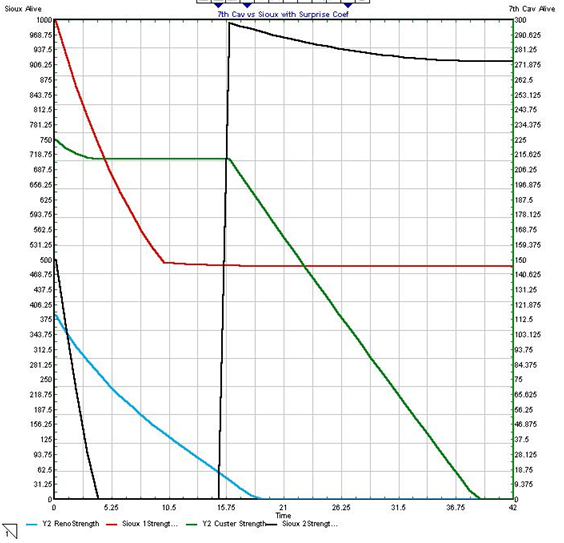
\includegraphics[scale=0.4]{fig6b.png}
\caption{$7^{th}$ Cavalry Attacks Divided Between Reno and Custer with Surprise Coefficient}
\label{fig6b}
\end{center}
\end{figure}

\begin{table}
\begin{center}
\begin{tabular}[h!tp]{ccccc}
\hline
\textbf{Time (minutes)} & \textbf{Reno Strength} & \myalign{p{3cm}}{\textbf{Sioux 1 Strength (vs. Reno)}} & \textbf{Custer Strength} & \myalign{p{3cm}}{\textbf{Sioux 2 Strength (vs. Custer)}} \\
\hline\hline
0 &	115 &	1000 &	225 &	500 \\
1 &	105 &	931 &	220 &	365 \\
2 &	96 &	862 &	216 &	230 \\
3 &	87 &	799 &	214 &	98 \\
4 &	79 &	742 &	213 &	0 \\
5 &	72 &	689 &	213 &	0 \\
6 &	65 &	642 &	213 &	0 \\
7 &	58 &	599 &	213 &	0 \\
8 &	52 &	560 &	213 &	0 \\
9 &	47 &	525 &	213 &	0 \\
10 &	42 &	494 &	213 &	0 \\
11 &	37 &	492 &	213 &	0 \\
12 &	32 &	491 &	213 &	0 \\
13 &	27 &	490 &	213 &	0 \\
14 &	22 &	489 &	213 &	0 \\
15 &	17 &	488 &	213 &	0 \\
16 &	12 &	487 &	213 &	994 \\
17 &	7 &	487 &	203 &	987 \\
18 &	2 &	487 &	193 &	981 \\
19 &	0 &	486 &	183 &	975 \\
20 &	0 &	486 &	174 &	969 \\
21 &	0 &	486 &	164 &	963 \\
22 &	0 &	486 &	154 &	958 \\
23 &	0 &	486 &	145 &	953 \\
24 &	0 &	486 &	135 &	949 \\
25 &	0 &	486 &	126 &	944 \\
26 &	0 &	486 &	116 &	940 \\
27 &	0 &	486 &	107 &	936 \\
28 &	0 &	486 &	98 &	933 \\
29 &	0 &	486 &	88 &	930 \\
30 &	0 &	486 &	79 &	927 \\
31 &	0 &	486 &	70 &	924 \\
32 &	0 &	486 &	60 &	922 \\
33 &	0 &	486 &	51 &	920 \\
34 &	0 &	486 &	42 &	918 \\
35 &	0 &	486 &	33 &	916 \\
36 &	0 &	486 &	24 &	915 \\
37 &	0 &	486 &	15 &	914 \\
38 &	0 &	486 &	5 &	913 \\
39 &	0 &	486 &	0 &	913 \\
\hline
\end{tabular}
\end{center}
\caption{$7^{th}$ Cavalry Attacks Divided into 2 Groups with Surprise Coefficient (data)}
\label{tab6b}
\end{table}

When the Sioux counterattack, Custer is annihilated within 24 minutes of the attack.  The end result of the combined battles is 1399 Sioux remain and the $7^{th}$ Cavalry is annihilated.  When using the Lanchester Square Law, having an advantage in numbers is generally more important than killing efficiency.   The recalculated results from Requirements 4 and 5 with a surprise coefficient provide an indication of how much of an improvement in killing efficiency would be required to overcome being outnumbered in an aimed fire situation.

\section{Exploration}
\subsection{Requirement 7}
Using Equations (1.3) and fixing $a = 0.01$, we were asked to experiment with values of $b$ and tactics (e.g. attacking the Sioux sequentially 500 at a time) in order to find a combination of surprise, technological superiority (here represented by $\frac{b}{a}$) and tactics that produces an outcome where the $7^{th}$ Cavalry is not annihilated. We were then asked to summarize the scenario described above and comment on its plausibility.   

One assumption made was that LTC Custer had a surprise factor of 20 which increased his kill efficiency from 0.03 to .6 ($20\times 0.03$) for the entire simulation.  Another assumption was that Capt. Benteen Forces (260) joined MAJ Reno 25 minutes after MAJ Reno began to fight the 1000 Sioux (Green). The final assumption was selecting random times at which the additional waves of 500 Indians began their counter attacks (Purple). Figure \ref{fig7a} shows the results of the simulation.
%TODO: re-do fig7a
\begin{figure}[h!tp]
\begin{center}
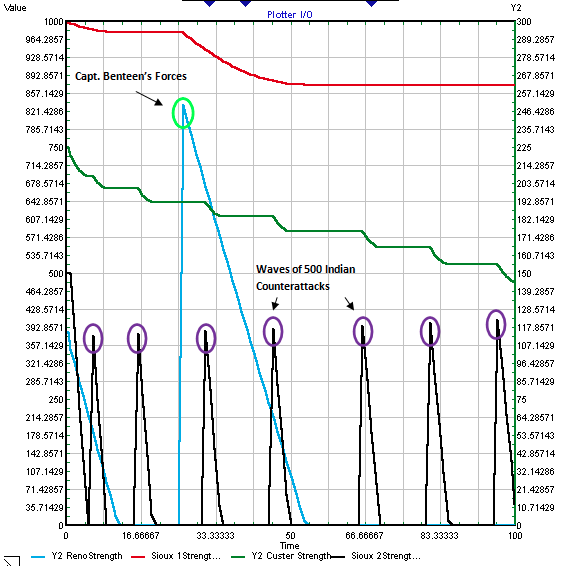
\includegraphics[scale=0.6]{fig7a.png}
\caption{$7^{th}$ Cavalry attacks Sioux variations}
\label{fig7a}
\end{center}
\end{figure}

Overall, the battle lasted 100 minutes. Based on the data collected after running the simulation the following conclusions were made (see Table \ref{tab7a}).

\begin{table}
\begin{center}
\begin{tabular}[h!tp]{ccc}
\hline
\textbf{Time	LTC} & \textbf{Custer Strength} & \textbf{Sioux Strength} \\
\hline\hline
0	& 225 &	500 \\
4	& 209 &	104 \\
6	& 208 &	375 \\
9	& 200 &	2 \\
16	& 200 &	378 \\
19	& 193 &	21 \\
31	& 192 &	385 \\
34	& 184 &	40 \\
46	& 184 &	390 \\
49	& 175 &	61 \\
66	& 175 &	395 \\
69	& 166 &	82 \\
81	& 165 &	401 \\
85	& 155 &	10 \\
96	& 155 &	407 \\
100	& 145 &	41 \\
\hline
\end{tabular}
\end{center}
\caption{$7^{th}$ Cavalry attacks Sioux variations (data)}
\label{tab7a}
\end{table}

The long term effect of allowing the Native Americans to be armed with rifles and mounted on horses was that it allowed a technological edge over the $7^{th}$ Cavalry. In terms of the assumptions made, the $7^{th}$ Cavalry had a training edge and fought in a coordinated manner that gave them a better killing efficiency.  Adding in Capt Benteen’s Forces, which contributed Gatling guns, also contributed to some degree to the survival of LTC Custer and his forces. The surprise tactic that was introduced into the model was having waves of 500 Indians counterattack at random times throughout Custer’s battle. This allowed for the entire 5,000 Sioux warriors to be accounted for.   With this in mind we increased LTC Custer’s killing efficiency from 0.03 to 0.6 ($20\times 0.03$). This allowed LTC Custer to gradually lose men throughout the battle but not to be completely annihilated.  Increasing the kill efficiency of LTC Custer allowed for Custer to survive the battle even with the waves of 500 Indians being introduced into the model.   

Given the assumptions above, increasing the kill efficiency for LTC Custer seemed plausible. The reason is because the arsenal of LTC Custer's forces increased from just single shot carbines to  include repeater rifles and gatling guns. On the other hand, the surprise tactic of introducing waves of 500 makes this scenario seem implausible. the noise from each chain of battles would alarm more Indian forces to enter the battle earlier then what we assumed. The ability to isolate small groups of the counter attack forces would be extremely difficult. For these reasons, this scenario can be seen as implausible.  

Lanchester’s Linear Law applies to unaimed fire into an enemy-occupied area. The rate of attrition depends on the density of the available targets in the target area as well as the number of weapons firing. For example, if two forces occupying the same land area and using the same weapons fire randomly into the same target area, they both will suffer the same rate and number of casualties, until the smaller force is eventually eliminated. However, Lanchester’s Square Law specifies the casualties a firing force will inflict over a period of time, relative to those inflicted by the opposing force. The Square Law is only used to predict outcomes and casualties by attrition. With firearms engaging each other directly with aimed fire from a distance, they can attack multiple targets and can receive fire from multiple directions. The rate of attrition now depends only on the number of weapons firing. The power of such a force is proportional not the number of units it has, but the square of the number of units. For these reasons, the square law applies.   

\subsection{Requirement 8}
We were asked to make one improvement to model (1.3), update our Extend model to reflect the new model, and report the outcomes. The improvements that were made to model (1.3) were in an effort to make the model more historically accurate. One assumption made was that 225 men under LTC Custer attacked the initial 500 Sioux 45 minutes after MAJ Reno began to attack 1000 Sioux. Another assumption was that during LTC Custer’s battle, 1000 Indians Counterattacked 65 minutes after Custer attacked the initial 500 Sioux.  The last assumption was that Capt. Benteen Forces (260) joined MAJ Reno 25 minutes after MAJ Reno began to fight the 1000 Sioux. Figure \ref{fig8a} shows the results of the simulation.
%TODO: re-do fig8a
\begin{figure}[h!tp]
\begin{center}
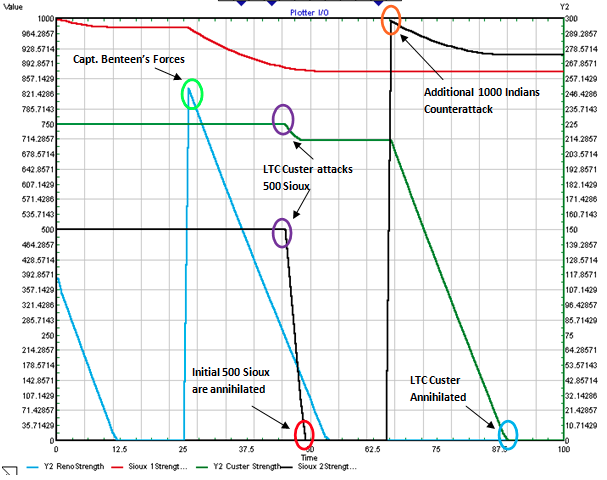
\includegraphics[scale=0.5]{fig8a.png}
\caption{$7^{th}$ Cavalry attacks Sioux, additional variations}
\label{fig8a}
\end{center}
\end{figure}

The overall battle lasted 88 minutes. Based on the data collected after running the simulation the following conclusions were made. At 48 minutes into the battle LTC Custer’s strength was 214 personnel while the Sioux Strength was at 98 personnel.  At 66 minutes, LTC Custer’s strength was 213 personnel and the Sioux Strength was at 994 personnel thanks to the additional 1000 Indians that where counterattacking LTC Custer’s efforts. At the end of the battle, LTC Custer’s Strength was 5 personnel while the Sioux Strength was 913 personnel. Although the improvements allowed both MAJ Reno and LTC Custer to last longer in the overall battle they eventually were annihilated.

\subsection{Requirement 9}
Modern campaign planning has been greatly influenced by technical superiority and unbalanced force ratios.  Known technical superiority or force size advantage has led to the disadvantaged side leveraging unconventional tactics and avoiding a traditional style of combat, symmetric warfare, where large numbers of troops face each other and battle over a parcel of land.  Knowledge one is out-manned and out-gunned by their opponent has directly led to finding alternative methods of fighting and inflicting casualties.  The extreme technical superiority and large size of United States forces has encouraged the use of unconventional tactics, asymmetric warfare, such as roadside bombs, attacking civilians, use of human shields, and other guerrilla and terrorist attacks.

Shock and awe similar to what was used by the Spaniards is common in modern warfare. The United States used this tactic in Baghdad and in WWII, with goals being to deter the enemy from fighting or to convince the enemy to surrender.  A disadvantaged side can also try to employ shock and awe, as evidenced by the attacks of 9-11.

The doctrine, \emph{Shock and Awe: Achieving Rapid Dominance}, was written by Harlan K. Ullman and James P. Wade and is a product of the National Defense University of the United States. This is a military doctrine based on the use of overwhelming power, dominant battlefield awareness, dominant maneuvers, and spectacular displays of force to paralyze an adversary's perception of the battlefield and destroy its will to fight.  Inasmuch, this tactic can take many forms and can be used effectively by forces large and small.

As evidenced in many of the ExtendSim models in this project, technological superiority combined with sound tactics (e.g., divide and conquer) can result in battles won even in the face of superior force strength.  If, however, technological superiority is not sufficiently great or cannot be sustained, force strength will likely prevail.

\end{document}